%! Author = adam
%! Date = 28.02.21

\chapter{Ion Beam Methods}\label{ch:ion-beam-methods}
\epigraphfontsize{\small\itshape}
\epigraph{ ``It was quite the most incredible event that has ever happened to me in my life. It was almost as incredible as if you fired a 15-inch shell at a piece of tissue paper and it came back to hit you''}{--- \textup{Ernest Rutherford}, \cite{2}}
Now lets see if instead of penetrating a sample, we scatter away from it.
An important term here is the \textit{scattering cross-section}, which is the probability of an ion-solid interaction.
\textit{The differential cross-section}  gives us a measure of either the probability of transferring energy $E$ in range $[E, E + dE]$ or the probability of scattering into angle $[\theta, \theta + d\theta]$. If we integrate the differential cross-section overl all $\theta$, we recieve a value called the \textit{total cross-section} Most of the time the scattering cross section is given in units of mm$^2$.
A diagram to better understand the microscopic scattering cross section is found in Figure~\ref{fig:rutherford}.

\begin{figure}
	\centering
	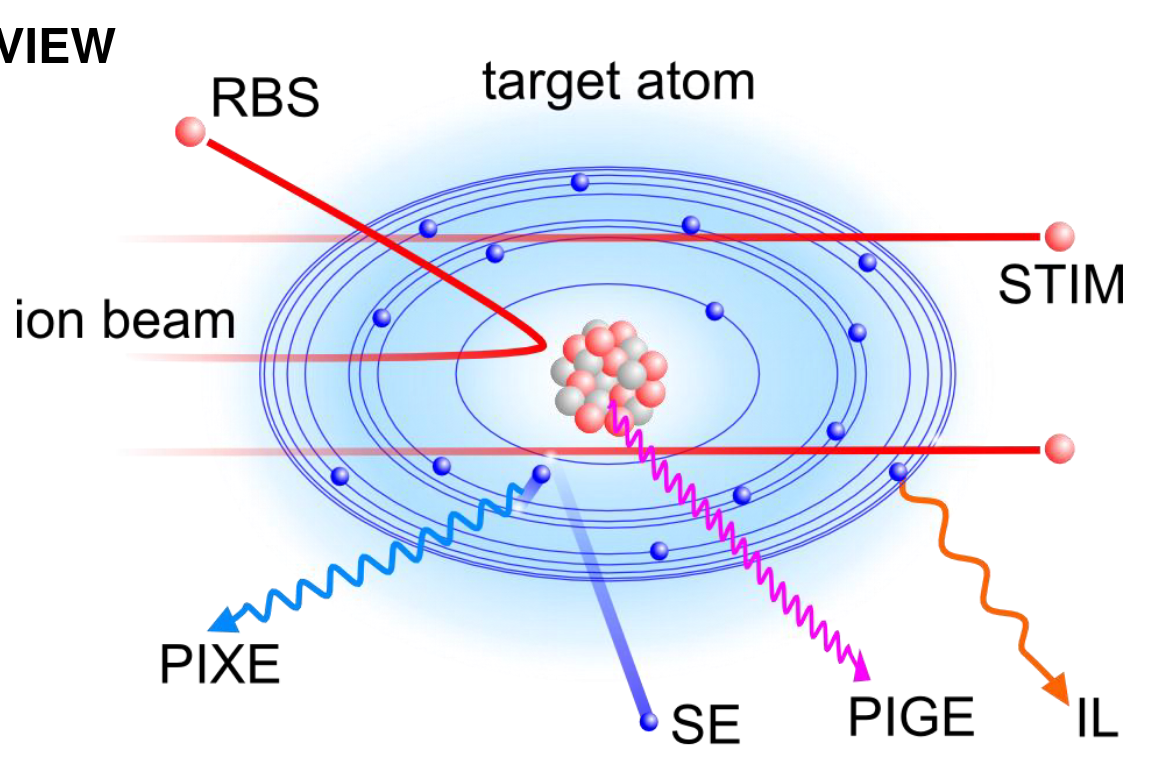
\includegraphics[width=0.7\linewidth, height=6.5cm]{overview}
	\caption{Various reactions of an ion beam hitting a target atom. The target atom has a nucleus and atomic shell, from which we can receive valuable information depending on how the beam interacts. STIM is the transmission of the ion through the sample, used in scanneing tunneling microscopy. }
	\label{fig:over}
\end{figure}
In this chapter we want to see how we can use ion beams to analyze samples.
These techniques are used in Leipzig, and we can see how some of these classical methods of ion beams can be used for quantum technologies.
First we need to see the difference between electron and proton radiation.
With electrons, we normally have large angle scattering, as well as not so deep range into the sample.
For protons, at the beginning of the trajectory there is not as much straggling as the electron, followed by a Bragg peak at the end.
Along the path there is very limited straggling, and the spatial resolution is high in comparison to the electron beams.
The penetration depth is also comparatively larger.
Now we want to see and discuss protons interacting with a solid in order to do analysis of the solid.
A general overview of the different ion beam methods is given in Figure \ref{fig:over}



\section{Rutherford Backscattering - RBS}\label{sec:rutherford-backscattering---rbs}
In RBS, the ion interacts with the nuclei of the target atom.
We discussed in earlier chapters rutherford scattering, which this is a derivative as such.
Imagine an ion with mass $M_1$, initial velocity $v_0$, corresponding to initial energy $E_0$ hurtling towards an atom at rest with mass $M_2$.
This ion, keep imagining, is on a direct collision course with the atom, as seen in Figure~\ref{fig:RBS}.
The resulting scattering of the projectile will result in a velocity $v_1$, and corresponding energy $E_1$, while the target nucleus now has velocity $v_2$ corresponding to energy $E_2$.
Let's say we do not know the target solid, and thus the mass $M_2$.
We can use the kinematic factor $\kappa $, defined as $\kappa = \frac{E_0}{E_1}$.
This turns out to be a function of the mass of the target atom $M_2$ and $M_1$, as well as the scattering angle $\theta$.
In order to make the indices simpler, lets switch to $M_p $ for mass of projectile, and $M_t$ as mass of target.

\begin{equation}
	\kappa = \left[ \frac{\sqrt{1 - \left( \frac{m_p}{m_t} \sin\theta \right)^2}  + \frac{m_p}{m_t}\cos\theta}{1+\frac{m_p}{m_t}} \right ]
\end{equation}
This equation is valid for $E_0 < U_c$, i.e., the coulomb potential, because there is no nuclear reaction therewith, which we do not want with these kinds of experiments.
In deriving $\kappa$, we see that it is a function of $M_p$, $M_t$, $\theta$! This means that if we were to have a detector to determine the angle of scattering, and we know the mass of the projectile, then we can determine the mass of the target atom.
This is exactly what Rutherford did, as he found that the charge needed to accomplish this reflection was approximately 100 times the charge of the electron, which is in nearly the atomic number of gold, the target atom he was using.
It is hard to put the detector at directly $180^{\deg}$, so sometimes we use ring detectors, or simply but the detector at $170^{\deg}$.
\begin{figure}
	\centering
	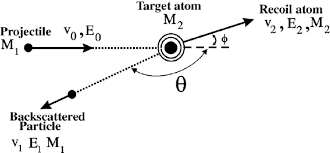
\includegraphics{RBS.png}
	\caption{A diagram of Rutherford Backscattering}
	\label{fig:RBS}
\end{figure}
\subsection{Cross Section}
If the cross section of the RBS event is low, then we will not see any scattering occur, even at very low scattering angles.
The probability of the scattering event is given by the cross section $\sigma$ (area of target atom), number of scattering atoms $N$ per overall area $A$:
$$ P = \frac{N}{A}\sigma$$
For the number of scattering events per unit time, $I$ in terms of this probability and the incident beam current $I_0$ as $I = I_0 P \rightarrow = \frac{I_0 N}{A} \sigma$.
If we assume Rutherford scattering, we just have Coulomb scattering, i.e., there is no screened potential that we need to account, since we are interacting directly with the target nuclei.
If $M_t << M_p$, then the \textit{differential cross section} can be written as:
\begin{equation}
	\frac{d\sigma}{d\Omega} = \left( \frac{Z_pZ_t e^2}{16\pi\epsilon_0 E}\right)^2 \frac{1}{\sin^4 \left(\theta / 2 \right)}
\end{equation}
This is the singularity for when the cross section is zero implies that the projectile never comes close to the target, but in this case it also never penetrates the electron cloud surrounding the nucleus either.
The pure Coulomb formula for the scattering cross section must be correct for this screening effect, which means it becomes more important as the energy of the projectile decreases.
It is important to note the following proportionality of the differential cross section.
$\propto (Z_p Z_t)^2 $ means that the projectile with higher charge ( or atomic mass) are advantageous, i.e., Helium is then better than just Hydrogen.
$\propto E^{-2}$ means that an increase in $E$ leads to a decrease in yield.
This is not good because we want to measure the most possible number of backscattered ions.
$\propto 1 / \sin^4 \theta / 2$ means that a decrease of yield with increasing $\theta$.
An example for a layered example of TiO$_2$ and Sapphire (Al$_2$O$_3$), and using literature values of $\kappa _{Ti} = 0.7171$, $\kappa_O = 0.3626$, $\kappa_{Al} = 0.5526$.
Fitting the values, we can determine the thickness of the layer of titanium oxide to be about $720$nm.


\section{PIXE}
Instead of interacting with the nucleus of the target atom, \textbf{P}article \textbf{I}nduced \textbf{X}-Ray \textbf{E}missions,  or \textbf{PIXE}, is a characteristic of scattering in which the ion beam interacts with the atomic shell of the target atom.
For interactions with the nuclei, this \textbf{P}article \textbf{I}nduced \textbf{G}amma-Ray \textbf{E}missions, or \textbf{PIGE}.
A process that occurs simultaneously with PIXE is the secondary electron emission which one can also analyze.
At higher electronic orbitals we have a phenomena called ion luminescence, where because of the higher orbital interaction, photons with wavelengths in the visible light range are emitted.
PIXE is used by geologists, archaeologists, and even art historians since it is a non-destructive elemental analysis technique that can help answer questions of provenance, dating, and authenticity.
Three types of spectra can be collected form a PIXE experiment: X-ray, Rutherford backscattering, and Proton transmission spectrum.
For X-ray emission, quantum theory states that orbiting electrons must occupy discrete energy levels in order to be stable.
If we bombard a sample with high enough energy ions (MeV protons), then the inner shells of the target atom will become ionized.
Outer shell electrons drop down to replace inner shell vacancies, however only the certain transitions are allowed, thus X-rays of these characteristic energy of the element are emitted.
A detector is used to record and measure these X-rays.
Only elements heavier than fluorine can be detected.
For a quantitative approach, the characteristic equation for the yield (measured inside the detector) is given in the lecture is written as follows:
\begin{equation}
	Y_X (Z) = \frac{N_A \omega_Z b_X \epsilon N_I c_Z}{A_Z} \int_{E_0}^{E_t} \frac{\sigma_Z (E) T_Z(E)}{S(E)} dE
\end{equation}
where $N_A $ is Avogadro number,
$\omega_Z$ the fluorescence yield of transition of element Z,
$b_X$ is the branching ratio, i.e.,  relative Intensity of line in the series of lines,
$\epsilon$ is the efficiency of the detector,
$N_I$ the number of incident particles ,
$c_Z$ the mass concentrations of emitting element Z,
$A_Z$ the mass number of emitting element Z,
$E_0$ the initial energy of incident particles,
$E_t$ the energy of ions after transmission through the sample or $E_{tmax} = 0$,
$Z(E)$ the ionization cross section,
$S(E)$ the stopping of the sample,
$T_Z(E)$ the transmission factor of the x-ray line X.

\section{Ion Beam Induced Charge}
Every charged particle (10 eV) deposits energy into a solid via Coulomb interaction.
This will create electron holes / pairs in the solid that we can use, for example quality checks in semiconductor devices.
Let's assume we have a solid and we are hitting it with an ion beam in the range of MeV.
There will be penetration into the solid and during the Coulomb interaction, we will produce energy transfer into the electrons of the solids, and thus holes/pairs in the neighbourhood of the ion path.
We will thus have a cone shaped plasma inside the solid created by depositing energies and thus producing electrons and holes (positively charged since electrons have left).
If we are using MeV, then we have a depth within the sample of a few $\mu$m and the cone of plasma will be much smaller in radius than the range.
\subsection{Klein Model}
The model developed by Klein, states that the amount of energy needed to create an electron-hole-pairs (EHP), is largely independent of the energy of the sample and type of ionizing radiation from your ion beam.
For example, for silicon we have an energy of 3.26 eV at 300k, and we use an ion at 1 MeV, we will produce lots of EHP, and create a large amount of free charge carriers.
The consequence of the Klein model is that if we use MeV ions on a single ion track, we can produce measurable signals found in pulse height spectrum (PHS).
This is done fore example, by irradiating a sample (an silicon integrated circuit) with ions in MeV region and connect the sample with a charge counter, then we get pulses in the form of a historgram, of events where we produce EHP.
The average of this histogram is then proportional to the change in the electrode.Can help in finding the quality or efficiency of a semiconductor device.

\subsection{Gunn Theorem}
\begin{wrapfigure}{r}{0.5\textwidth}
	\centering
	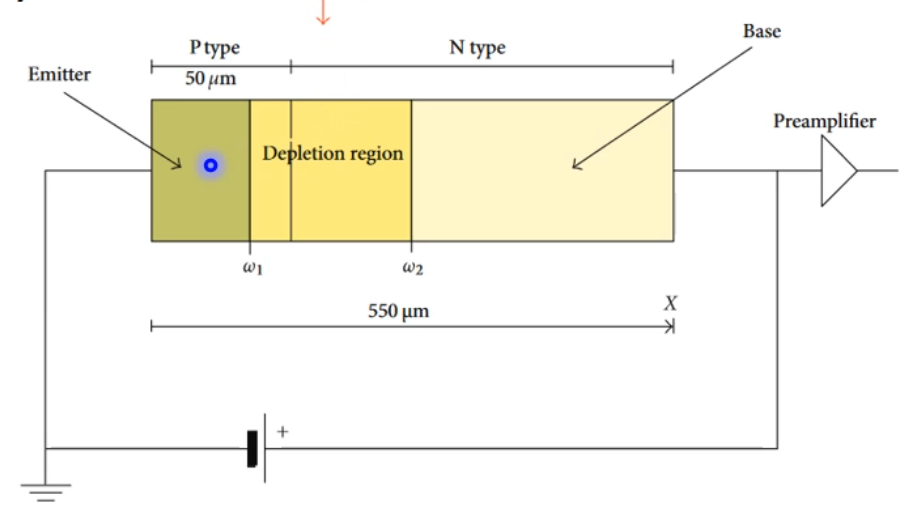
\includegraphics[scale=0.25]{gunndevice}
	\caption{A typical semiconductor diode used to demonstrate Gunn Theorem. A 5 MeV proton beam hits the sample normal to the top of the device. The device is connected to some voltage to suck away the free charge carriers produced by the proton beam. Some electronics like the preamplifier can be used to count the pulses and thus produce a histogram spectrum. }
	\label{fig:semidevice}
\end{wrapfigure}
Developed in 1964, Gunn Theorem, observed by J.B. Gunn in materials with energy band structures, and is a quantitative approach to the Klein model.
We can calculate the expected current at a position within a device given an impact of an ion beam using the equation below.
An example of such a semiconductor device is given in Figure~\ref{fig:semidevice}.
$$ I_i = -q \vec{v} \frac{\partial \vec{E}}{\partial V_i} $$
We have a charged particle, for example a proton beam, $q$ in the above equation would be one, that is traveling wih some velocity $\vec{v}$.
We have then the electric field $\vec{E}$ derivative with respect to the bias voltage applied to the sample.
If we have lots of devices, with various connections, then we could calculate this current for the various junctions, which is indicated with the $i$ subscript.
This partial derivative, is Gunn's weighting field.
Now, we could also calculated the charge produced overtime with this current, $Q_i(t)$.
$$Q_i(t) = \int_0^t I_i(t^{\prime}) dt^{\prime} = -q \int_{r_l}^{r_F} \frac{\partial \vec{E}}{\partial V_i} d\vec{l} = q \left[ \frac{\partial \psi}{\partial V_i} |_{r_F} - \frac{\partial \psi}{\partial V_i} |_{r_l} \right]$$
This is just the integration of the current over time, since charge is current over time.
We could then transform the integral to integrate over the length of the sample using Gauss theorem, since the potential of the electric field has the relation $\nabla \psi = -E$.
In the end we are able to get a relationship between the incident beam and the charge (or current) within the diode.
In the continous case, we have
$$ Q_i(t) = -q \int_0^t dt^{\prime} \int_{\Omega}  d^3 r \left[ x(\vec{r},t) \vec{v}_x (\vec{r}) \frac{\partial\vec{E}}{\partial V_i} \right]$$
\newpage
\begin{wrapfigure}{l}{0.5\textwidth}
	\centering
	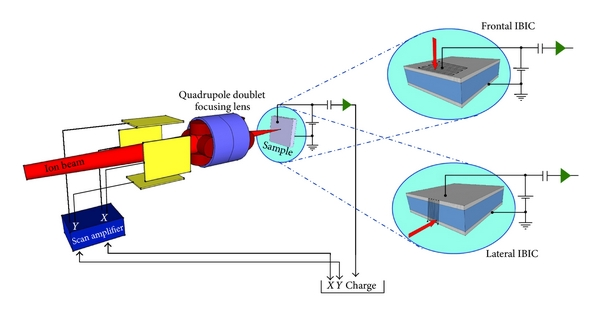
\includegraphics[scale=1.5]{ibic.jpg}
	\caption{Scheme of the IBIC setup. A MeV ion beam from an accelerator is focused by a quadrupole lens system and scanned over the sample surface using two sets of magnetic or electrostatic plates. The insets on the right sides show the two irradiation geometries: from the top (frontal IBIC) and from the side (lateral IBIC) of the device under analysis. Each incident ion generates a measurable charge pulse, which is amplified and processed by a standard charge sensitive electronic chain. The data acquisition system acquires and stores every event along with the coordinates of the ion. \cite{5}}
	\label{fig:ibicmic}
\end{wrapfigure}
These methods can be used for microscopy, which can be seen in Figure~\ref{fig:ibicmic}.
If we scan the beam over the sample, we can get an image if the charge creation within the sample from the incident beam creating charges.
The histogram will then be the amount of charge one gets at a certain position, based on the scanning of the beam.
This will give us insight into the quality of the device, and is often used to check the quality of integrated circuits.
It is also possible to use this technique for the detection of single ions, which is especially useful for quantum computing.
We know that quantum computing needs to be scalable, so if we are to use ion implantation, we must be sure that we are inserting single ions correctly.

\section{Summary}
There are of course many other forms of scattering, some of which are not covered in detail here but are of note.
There is Elastic Recoil detection (ERD), which is used to obtain elemental concentration depth profiles in thin films.
Nuclear reaction analysis (NRA) is a method of nuclear spectroscopy to determine concentration versus the depth distributions for certain target chemical elements in a solid thin film.
\begin{myitemize}
	\item RBS is based of the elastic scattering of the ion with a target atom (ion-nucleus interaction)
	\item PIXE and PIGE are interactions of the ion with the target electron orbitals, the latter being of higher orbital interactions
	\item IBIC Klein Model, creating EHP is largely independent of sample energy as well as type of ionizing radiation.
	\item The methods of precise ion beams are good for quality assessment, or for implanting ions, but also for detecting single ions that wer previously implanted.
\end{myitemize}
